\documentclass[10pt,twocolumn,letterpaper]{article}
 \pdfoutput=1
\usepackage{cvpr}
\usepackage{times}
\usepackage{epsfig}
\usepackage{graphicx}
\usepackage{amsmath}
\usepackage{amssymb}
\usepackage{bm}
\usepackage{subcaption}
\usepackage{slashbox}
\usepackage{color}
\usepackage[english]{babel}
\usepackage[linesnumbered,ruled,vlined]{algorithm2e}
\usepackage[breaklinks=true,bookmarks=false]{hyperref}


\newcommand{\argmin}{\operatornamewithlimits{argmin}}
\cvprfinalcopy

\def\cvprPaperID{16} % *** Enter the CVPR Paper ID here
\def\httilde{\mbox{\tt\raisebox{-.5ex}{\symbol{126}}}}
\begin{document}
\title{DeepTrack: car trajectory prediction for autonomous driving}

\author{Di Wu, Zhennan Wang, Yi Tang,  Wenbin Zou, Xia Li\\
Shenzhen University\thanks{Shenzhen Key Lab of Advanced Telecommunication and Information Processing, College of Information Engineering, Shenzhen University.}\\
{\tt\small dwu,...@szu.edu.cn}}
\maketitle
%%%%%%%%% ABSTRACT
\begin{abstract}


\end{abstract}
%%%%%%%%% BODY TEXT
%%% Andrje Karpathy's blog: http://karpathy.github.io/2016/09/07/phd/
%%% Another great resource on this topic is Tips for Writing Technical Papers from Jennifer Widom.
%%% https://cs.stanford.edu/people/widom/paper-writing.html
\section{Introduction}

\begin{figure}

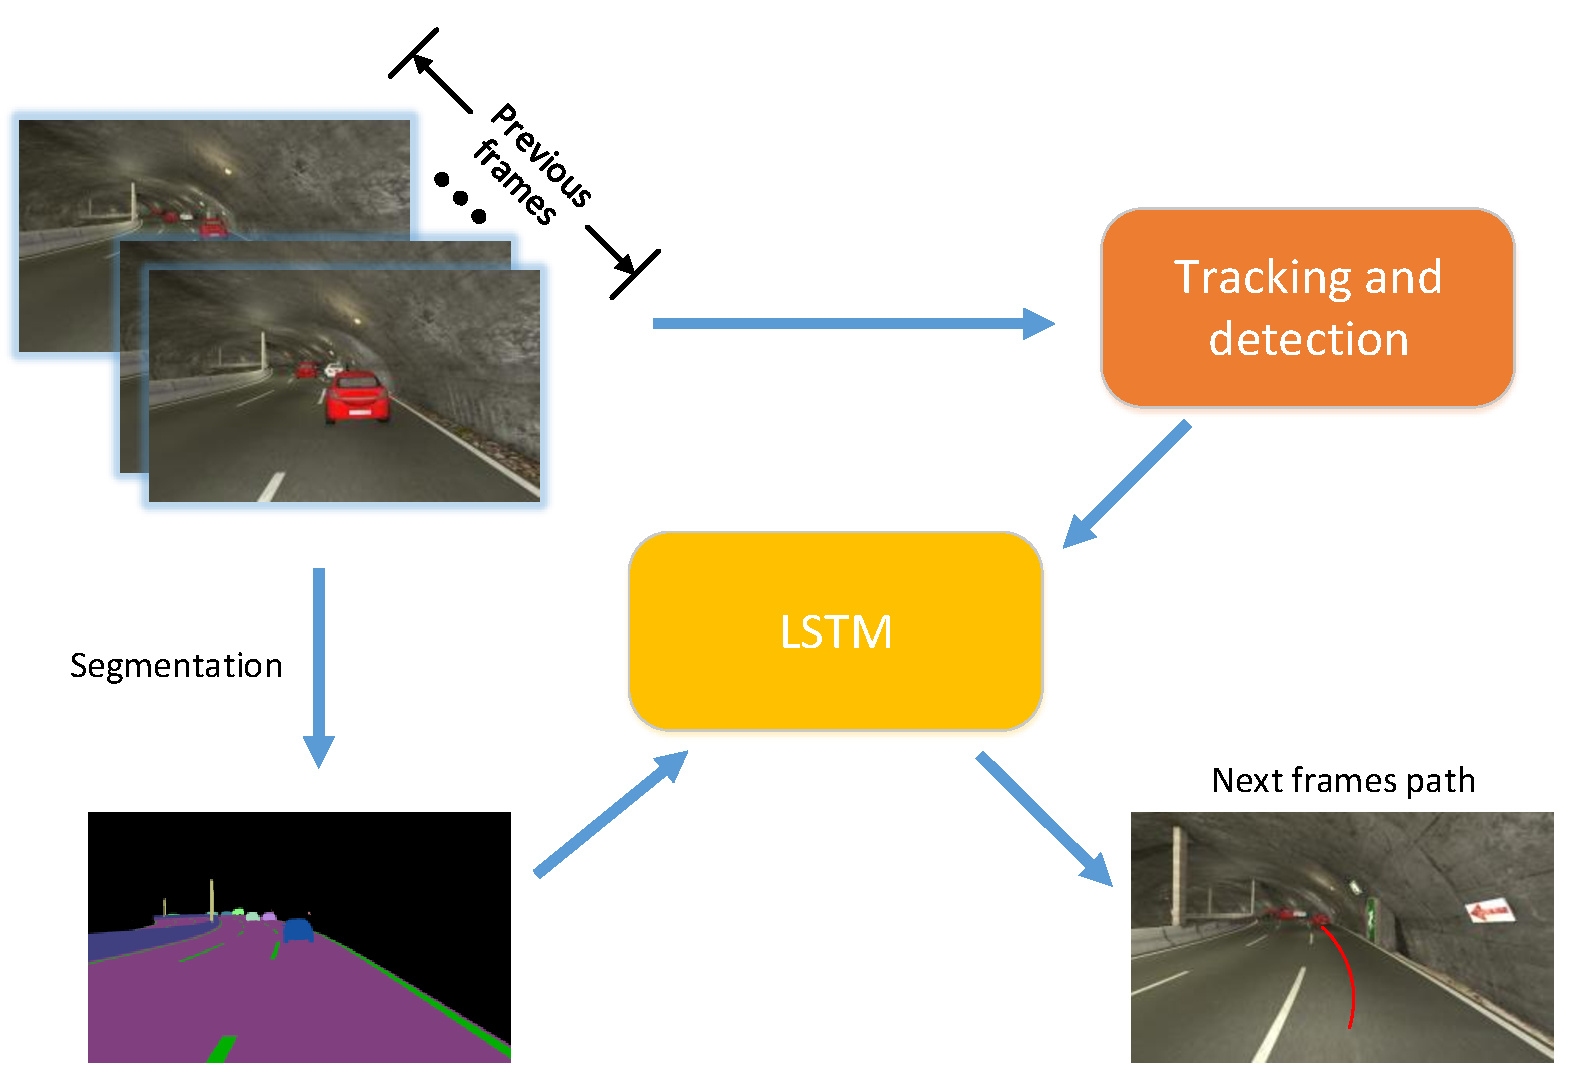
\includegraphics[width=8.8cm]{pool_figure}
\caption{pool figure}
\label{figure10}
\end{figure}

\section{Related Work}

%%% TY: write related work for object detection, segmentation, instance segmentation

%%% DW: write related work for visual tracking
%%% DW: write related dataset for autonoumous driving

%% DW: (1)traditional segmentic segmentation dataset
%% DW: (2) synthetic dataset
%% DW: (3) temporal consistent dataset

Camvid dataset~\cite{Camvid} consists of a set of monocular images taken in Cambridge UK. However, only 701 images contain pixel-level annotations over a total of 32 categories (combining objects and architectural scenes).

Similarly, Daimler Urban Segmentation dataset~\cite{scharwachter2013efficient} contains 500 fully labelled monochrome frames for 5 categories.

KITTI benchmark suite~\cite{Geiger2013IJRR} provides a large a mount of images of urban scene from Karlsruhe, Germany, with ground truth data for odometry, object detection, tracking, scene flow and stereo benchmarks. However, a limited 430 labelled images are provided for semantic segmentation.

A common limitation of the aforementioned datasets is the bias introduced by the acquisition of images in a specific city. The LabelMe~\cite{russell2008labelme} project offers the solution by offering around 1,000 fully annotated images of urban environments around the world and more than 3,000 images with partial(noisy) annotations.

More recently, larger project are constructed:
Cityscapes dataset~\cite{Cordts2016Cityscapes} which consists of a collection of images acquired in 50 cities around Germany, Switzerland and France in difference seasons, and having 5,000 images with fine annotations and 20,000 with coarse annotations over a total of 30 classes.

The use of synthetic data has increased considerably in recent years within computer vision community. ~\cite{mueller2016benchmark} provides a synthetic dataset generation and online tracker evaluation. In~\cite{kaneva2011evaluation}, the authors used a photorealistic virtual world to evaluate the performance of image features under scene changes and image transformations. Synthetic data has also been used for skeleton joints estimation~\cite{shotton2013real}, allowing the classifier invariant to pose, body shape, clothing, etc.

A fine annotated images in Cityscape dataset requires on average 1.5 hours which is very labor intensive. Thus, the cost of scaling large project would required a prohibitive economic investment in order to capture images from a larger variety of countries, in different seasons and different traffic conditions. For these reasons, a novel synthetic dataset of urban scene called SYNTHIA~\cite{ros2016synthia} is proposed to use synthetic imagery that simulate real urban scenes in a vast variety of conditions and produce the appropriate annotations.
This dataset is a large collection of images with high variability due to changes in illumination, textures, pose of dynamic objects and camera view-points.p
%%% ZN: write related works for Recurrent Networks (used in the context of autonomous driving)

\section{Proposed Algorithm}

\section{Experiments}
\subsection{Dataset collection}
We collect car trajectory evaluation dataset based on the SYNTHIA~\cite{ros2016synthia} dataset.


\section{Conclusions}



\section*{Details of the Code}


\section*{Acknowledgment}

{\small
\bibliographystyle{ieee}
\bibliography{egbib}
}
\end{document}
